\documentclass{beamer}
\usepackage{amsmath}
\usepackage{amssymb}
\usepackage{mathrsfs}
\usepackage[LGR,T1]{fontenc}
\newcommand{\textgreek}[1]{\begingroup\fontencoding{LGR}\selectfont#1\endgroup}
\usepackage[utf8]{inputenc}
\usepackage{caption}
\usepackage{graphicx}
\graphicspath{ {tu/} }

\title[MATH 6380 Project 2]{Study on tree-based methods}
\subtitle{MATH 6380 project 2}
\author[C.Dong, T.C.LO, J.Xia]
{Chenyang,~DONG \and Tsz Cheung,~LO \and Jiacheng,~XIA}
\usetheme{CambridgeUS}
\usecolortheme{seahorse}
%%%
% The next block of commands puts the table of contents at the 
% beginning of each section and highlights the current section:

\AtBeginSection[]
{
  \begin{frame}
    \frametitle{Table of Contents}
    \tableofcontents[currentsection]
  \end{frame}
}
%
%%%

\begin{document}
\frame{\titlepage}

\begin{frame}
\frametitle{Outline}
\tableofcontents
\end{frame}

\section{Introduction}
\begin{frame}
\frametitle{Studying tree based methods...}
Why did we choose tree-based methods?
\pause
\begin{itemize}
\item We went through several methods.
\pause
\item Tree-based methods are straight-forward and easy to implement.
\pause
\item There are yet many improvement methods.
\pause
\item Studied the method on 2 datasets.
\end{itemize}
\end{frame}


%xia's part
\section{American Crime Dataset}
\begin{frame}
\begin{block}{The dataset}
This dataset and the preprocessing are the same as project 1.
\end{block}
\pause
\begin{exampleblock}{Goal for this dataset}
Do straightforward analysis and compare with Lasso (PJ 1).
\end{exampleblock}
\begin{alertblock}{What we found}
In terms of MSE, simple regression tree(0.11) slightly worse than Lasso(0.06); bagging, random forest and boosting even better(0.04, 0.02).
\end{alertblock}
\end{frame}

\begin{frame}
\frametitle{Visualize the results}
\begin{figure}[h]
  \centering
  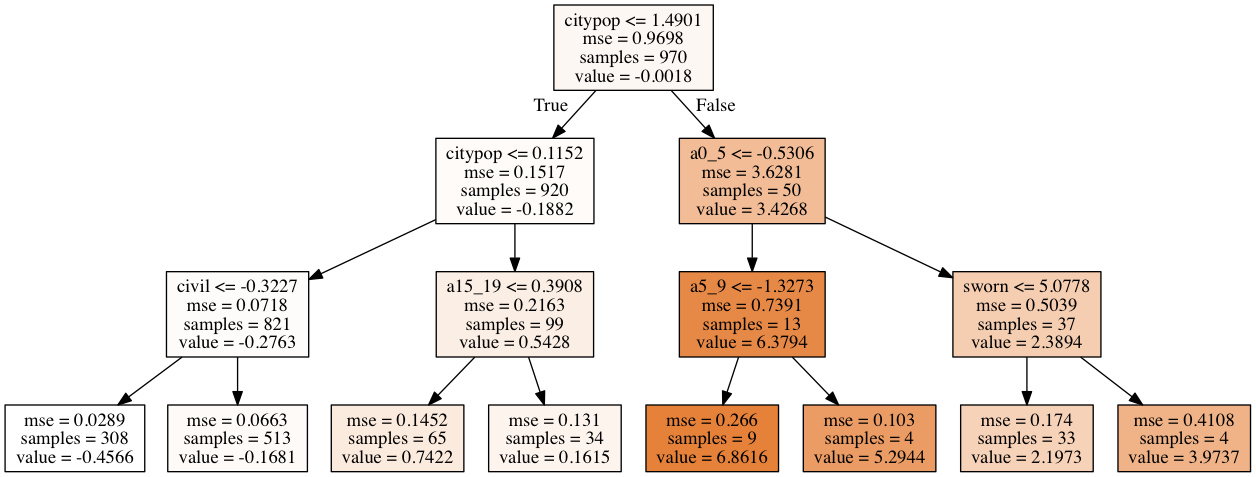
\includegraphics[width=10cm, height=4cm]{crime_treetu}
  \caption{Regression tree on crime data}
\end{figure}
\end{frame}

\begin{frame}
\frametitle{Boosting and random forests}
\begin{figure}
\centering
\begin{minipage}{.5\textwidth}
  \centering
  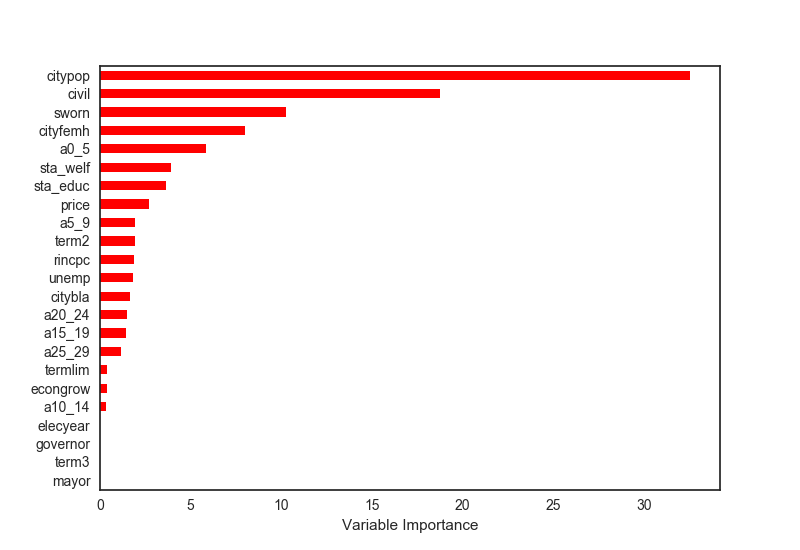
\includegraphics[width=.8\linewidth,height=4cm]{crime_boosttu}
  \captionof{figure}{Importance\\ from boosting}
  \label{fig:test1}
\end{minipage}%
\begin{minipage}{.5\textwidth}
  \centering
  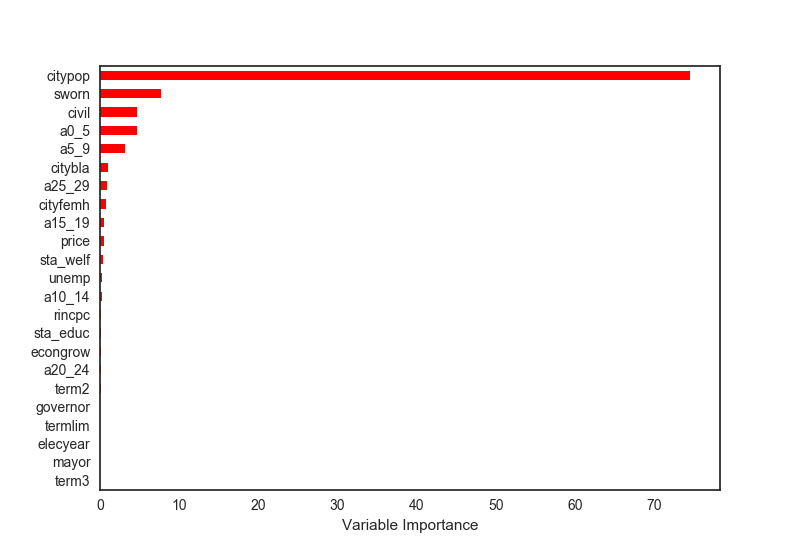
\includegraphics[width=.8\linewidth,height=4cm]{crime_randtu}
  \captionof{figure}{Importance\\ from random forest}
  \label{fig:test2}
\end{minipage}
\end{figure}
\end{frame}


%phil's part
\section{Kaggle: Binray Drug}
\begin{frame}
\frametitle{Variable Importance}
\begin{itemize}
\item The $\textbf{R randomForest}$ package optionally produces 2 additional pieces of information. One is called $\textbf{Variable Importance}$, a measure of the importance of the predictor variables.

\item It is based upon the mean decrease of accuracy in predictions on the out of bag samples
when a given variable is excluded from the model.

\item In this project, we define variables/predictors with $\%IncMSE > 0 $ as important variables, then select them as our predictors in our final model.	
\end{itemize}
\end{frame}


\begin{frame}
\frametitle{Importanct Variables in BinaryDrug}
The necessary calculations are carried out tree by tree as the random forest is constructed. Our experience has been that even though the variable importance measures may vary from run to run, the ranking of the importances is quite stable.
\begin{figure}[h]
	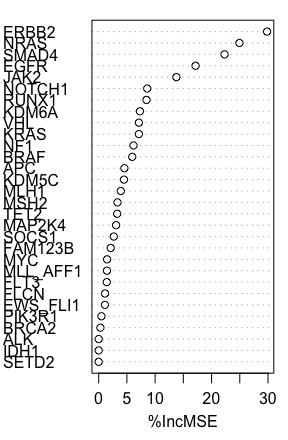
\includegraphics[width=5cm, height=6cm]{bagging_vi}
	\caption{I.V in BinaryDrug Data}
\end{figure}
\end{frame}



\begin{frame}
\frametitle{A potential variable selection method?}
\begin{itemize}
	\item We have tried $LASSO$ in this dataset. Bad.
	
	\item Somebody introduced $p-value$ selection. Kaggle $MSE$ = 3.08. Good.
	
	\item Can we do better using variable importance?
\end{itemize}
\end{frame}

\begin{frame}
\frametitle{some V.I related models}
\begin{itemize}
	\item V.I + $\textbf{MLR}$, Kaggle $MSE$ = 3.26057
	\pause
	\item V.I + $\textbf{Random Forest}$ with using all V.I, Kaggle $MSE$ = 3.23067\\
	\pause
	\item So sad. And I don't know why.
\end{itemize}
\end{frame}

\begin{frame}
\frametitle{However...}
\begin{itemize}
	\item What if we adapt a $\textbf{Random Forest}$ with $mtry$ slightly > \# of V.I ?
	\item Say in this Kaggle Competition, \# of V.I is 25, and we have tried $mtry = 25 \text{ to } 30$, all giving us $MSE$ lower than 3.10.
	\item (Maybe) this can be explained from that, using slightly more $mtry$ in each iteration can have a higher chance covering all those V.I when building  $\textbf{Random Forest}$.
\end{itemize}
\end{frame}


%who's part?
\section{Conclusion}
\begin{frame}
\frametitle{To conclude our work in PJ2...}
\begin{enumerate}
	\item Tree-based regression algos are suitable for these discrete-input, continous-output datasets.
	\item As a metric, $\textbf{Variable Importance}$ may not be useful for variable selection process.
\end{enumerate}
\end{frame}

\end{document}